

Many robotics applications consist of hybrid systems that exhibit both
continuous state flows and discrete state transitions. Common examples of hybrid
systems are contact-rich mechanisms such as legged robots and manipulators.
These mechanisms experience contact forces from their interaction with the
environment, causing them to undergo mode changes. 
%
For example, a humanoid bipedal robot consists of two potential contacts between
the legs and the ground.
%
If we only observe the contact forces exerted on one of the legs, we can find a
total of two modes~\cite{underactuated}.
%
In the first mode, called the \textit{swing mode}, the leg swings forward in the
air while balancing off of the other; this phase is governed by a continuous
dynamics with no contact forces on one of the legs. 
%
The second mode is the \textit{stance mode}, where the foot makes a persisting
contact with the ground and leverages the friction to balance the rest of the
mechanism.
%
These modes are connected by the \textit{heel strike guard}, where the leg
impacts the ground, causing a discrete state transition. 
%
Each one of these modes and their guard have a distinct dynamic behavior
governed by unique equations of motion, which can be written in a compact manner
as~\cite{goebel2009hybrid}
\begin{equation}
    \left\{
    \begin{array}{@{}c@{}}
        \smash[t]{\dot{x} \in f(x, u), \; x \in C,} \\
        \smash[b]{x^+ \in g(x, u), \; x \in D,}
    \end{array}\right.
    \label{eq:cont_and_guards}
\end{equation}
\noindent where $x \in \mathbb{R}^m$ is the state vector, and $u \in
\mathbb{R}^n$ is the input.
%
The set-valued mappings $f: \mathbb{R}^m \times \mathbb{R}^n \rightarrow
\mathbb{R}^m$ and $g: \mathbb{R}^m \times \mathbb{R}^n \rightarrow \mathbb{R}^m$
denote the flow and jump maps, respectively, where $C$ and $D$ are subsets of
$\mathbb{R}^m$ consisting of the feasible states under the flow and jump
rules, respectively. 
%
The notation $x^+$ indicates the state resulted by the jump rule $g$.


%
Controlling such multi-modal systems presents two main complications. 
%
First, it may be impossible to find a single policy that can achieve the desired
performance in all modes of the hybrid system.
%
A typical approach is splitting tasks into \textit{manipulation
primitives}~\cite{nonprehensile_survey,rodyman,lynch2003control}, such as
sliding, jumping, and toppling, where each primitive has a corresponding
dynamics and is assigned its own controller. 
%
\begin{wrapfigure}{r}{0.42\textwidth}
    \vspace{-9mm}
     \begin{center}
     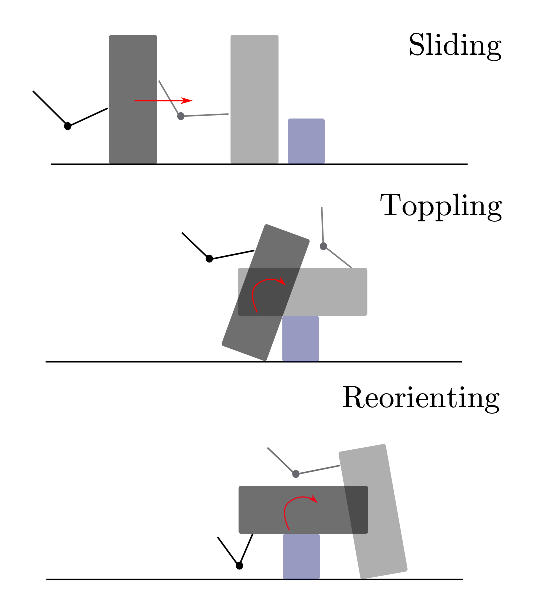
\includegraphics[width=0.43\textwidth]{primitives.eps}
     \vspace{-5mm}
     \end{center}
     \vspace{-2mm}
     \caption{Manipulation primitive sequence for manuvering a box past an obstacle}
     \label{fig:primitives}
     \vspace{-5mm}
\end{wrapfigure}
%
Consider the task of moving a box past an obstacle using a series of primitives
such as sliding, toppling and reorienting as shown in
Figure~\ref{fig:primitives}.
%
Each primitive has a region of applicability in the state space, where the
dynamics of that primitive describes the flow of the
system~\cite{lynch1999dynamic}.
%
Thus, manipulation planning involves identifying a successful primitive
sequence, such as the order of primitives shown in Figure~\ref{fig:primitives},
and stabilizing the system under each
primitive~\cite{erdmann1998exploration,yashima2003randomized}.  
%
This approach can be viewed as partitioning the state space and allocating a
control law in each subdomain that results in a successful transition to the
desired primitive until the goal state is reached~\cite{woodruff2017planning}.
%
However, the task of ordering the primitives and identifying the distinct
controllers in each state partition is done
manually~\cite{erdmann1998exploration,woodruff2017planning}, which does not scale
well to contact-rich systems with numerous modes. 
%
An example of such system is multiagent
manipulation~\cite{ashenafi2021nonholonomic}, which uses a group of robots to
cooperatively execute a task, such as maneuvering an object in space. 
%
As we change the number of robots establishing contact with the object, we find
new modes of the hybrid system.
%
A cooperative manipulation with $k$ potential contacts can have up to $2^k$
contact combinations. 
%
It is quite tedious and inefficient to manually identify and encode a successful
primitive sequence for various initial states and to find individual controllers
for each mode. 
%

To address this issue, we propose a data-driven approach for constructing
dynamic motion plans and stabilizing control laws for complex locomotion and
manipulation tasks that make and break contact.
%
Our framework leverages the \textit{mixture of experts} architecture from
supervised learning to infer multi-modal controllers for contact-rich systems.
% 
This approach \textit{automatically} learns the boundaries of the state
partitions and allocates the appropriate expert controller to each partition in
order to drive the system to the desired mode, and overall to the goal state.
%
We demonstrate the efficacy of this technique on the swing-up task of the
cartpole enclosed by wall barriers, both in simulation and real-world
experiments.

The second complication in the control of hybrid systems is that they operate in
an environment that is not known completely or modeled accurately.
%
For instance, a legged robot needs to be robust enough to be able to perform
satisfactorily on uneven terrain. Similarly, manipulators need to hold a firm
grip on objects of all textures.
%
There are techniques that combine tools from optimization, probability theory,
and machine learning to learn control strategies from inaccurate system models
or even unknown dynamics.
%
Model-free reinforcement learning is an example of a technique that relies on
repeated interactions with the unknown
environment~\cite{heess2017emergence,andrychowicz2020learning,lillicrap2015continuous}.
%
While this technique offers more flexibility on how the control policies are
inferred from unknown dynamics, they do not provide the physical structure
required to infer stability properties.
%
On the other hand, data-driven techniques trained in simulation, such as neural
passivity-based control (\textsc{NeuralPbc}~\cite{ashenafi2022robust} and
\textsc{Neural-Idapbc}~\cite{sirichotiyakul2022data}) offer more insight on the
stability of the system but strongly rely on the dynamical model.
%
The use of inaccurate models may lead to poor performance or even instability.
%

Bayesian learning (BL)~\cite{gal2016improving,thakur} offers an alternative
method to simultaneously combat model uncertainties while preserving the useful
stability properties in the \textsc{NeuralPbc} and \textsc{Neural-Idapbc} frameworks.
%
BL is typically used to characterize uncertainties of a dynamical system with a
stochastic model.
%
For instance, the framework presented in~\cite{sadigh2015safe} models
uncertainties caused by disturbances, such as the effect of wind gusts on
quadcopters, via Bayesian inference.
%
A similar approach is shown in~\cite{shen2022online, pmlr-v54-linderman17a}, where
a stochastic dynamical model is constructed via BL techniques, and utilized in
data-driven control synthesis executed in simulation. 
%
% For instance, BL is used to model uncertainties caused by disturbances, such as
% the effect of wind gusts on quadcopters and the motion of other vehicles in
% autonomous driving~\cite{sadigh2015safe}. 
%
% Nonlinear dynamics can be decomposed into segments of linear dynamics, and learn
% the linear dynamical units and their transition probabilities through
% BL~\cite{pmlr-v54-linderman17a}. 
% The authors of~\cite{shen2022online} perform Bayesian learning online to
% characterize time-varying kinematic and dynamical models of industrial robots.
% %
% Another approach to combating model uncertainties is to surpass the process of
% learning the stochastic model and instead directly learn the controller through
% BL. 
%
Adaptive control framework is provided in~\cite{fan2020bayesian}, where the
search for the control is given by a quadratic program that imposes
Lyapunov stability constraint for safety critical systems.
%
This technique uses BL to infer a controller through interactions with
unknown dynamics, while maintaining the algebraic structure of a stable system.
%
Inspired by this technique, we merge the structure and stability properties of
passivity-based control (PBC) with the robustness properties of BL.  


We present a unified framework that simultaneously combines data-driven
techniques and rigorously addresses model uncertainties using Bayesian learning.
%
% We aim to apply BL and develop an algorithm that finds a suitable probability
% distribution of the policy automatically.
%
In contrast to deterministic optimization, this approach provides a probability
distribution over the parameters of the controller instead of point
estimates, providing a way to reason about model uncertainties and measurement
noise during the learning process.
%
We first demonstrate the efficacy of this technique on smooth systems, such as
the simple pendulum and the inertia wheel pendulum, in simulation and real-world
experiment.
%
Then we extend the framework to contact-rich systems and evaluate its
performance on the rimless wheel, a simplified walking machine that still
represents the difficulties in controlling hybrid systems in uncertain
environments.
